\section{Results and Discussion}
\label{sec:results}

\paragraph{Results overview.}
PaCT removes the recurrent latent-unrolling bottleneck while preserving (and often improving) reasoning performance.
Across GSM8k, ProntoQA, and ProsQA, PaCT matches or exceeds Coconut while reducing training time by $3.2$--$4.7\times$
(Table~\ref{tab:main_results}), and these gains persist at larger model scales (Table~\ref{tab:performance_training}).
We then analyze \emph{why} PaCT works: (i) each latent stage contributes measurably to the final prediction
(Fig.~\ref{fig:accuracy_and_latent_stages}); (ii) PaCT promotes stage-wise specialization and scales well with depth
(Table~\ref{tab:latent_similarity}, Fig.~\ref{fig:accuracy_and_latent_stages}); (iii) latent trajectories exhibit
interpretable confidence dynamics (Table~\ref{tab:latent_confidence}, Fig.~\ref{fig:latent_examples});
and (iv) PaCT stabilizes internal dynamics relative to Coconut (Fig.~\ref{fig:icr}).
Finally, we validate a key architectural choice of restricting the cross-attention context for latent synthesis
(Sec.~\ref{subsec:context_length}).

\subsection{Experimental Setup}
\label{sec:experimental_setup}
To ensure a fair, direct comparison, we follow Coconut~\cite{hao2024training}, matching
model architectures, curriculum schedules, datasets, and optimization settings. This isolates the effect of PaCT’s
parallel latent reasoning from other confounders.
\vspace{-4mm}
\paragraph{Base models.}
Our primary experiments use GPT-2 Small (124M) as the base causal LM, without modifying the underlying Transformer
layers. To evaluate scaling with model size, we additionally run experiments using LLaMA-3B and LLaMA-8B as base
models (Table~\ref{tab:performance_training}). In all cases, PaCT is integrated on top of the base model with the
same module design.
\vspace{-4mm}
\paragraph{PaCT configuration.}
Unless stated otherwise, PaCT uses a fixed configuration: a latent query/codebook projection dimension of 128 and
4 attention heads for cross-attention. Latent synthesis uses a restricted context window consisting of the two most
recent hidden states; we ablate this choice in Sec.~\ref{subsec:context_length}.
\vspace{-4mm}
\paragraph{Curriculum training.}
We use Coconut’s multi-stage curriculum, progressively replacing textual CoT tokens with latent reasoning stages.
For GSM8k, we first fine-tune with CoT supervision for 25 epochs, followed by 25 epochs of curriculum-based latent
training. For ProntoQA and ProsQA, models are trained for 50 epochs under the same curriculum schedule as Coconut.
We set the maximum number of latent stages to 3 for GSM8k and 6 for ProntoQA and ProsQA.
\vspace{-4mm}
\paragraph{Optimization.}
We use AdamW with learning rate $1\times 10^{-4}$, weight decay 0.01, and effective batch size 128. We evaluate on
GSM8k (math), ProntoQA (deductive logic), and ProsQA (proof-oriented reasoning). Following prior work, the continuous
thought parameter is set to $c_{\text{thought}}=2$ for GSM8k and $c_{\text{thought}}=1$ for ProntoQA and ProsQA.
All experiments are conducted on a single node of H100 with four 80 GPUs.

\subsection{Parallel latent reasoning improves training efficiency without sacrificing accuracy}
\label{sec:efficiency}

\begin{table*}[t]
\centering
\begin{tabular}{lcccccc}
\toprule
\multirow{2}{*}{Method} 
& \multicolumn{2}{c}{GSM8k} 
& \multicolumn{2}{c}{ProntoQA} 
& \multicolumn{2}{c}{ProsQA} \\
\cmidrule(lr){2-3} 
\cmidrule(lr){4-5} 
\cmidrule(lr){6-7} 
& Acc. (\%) & Train Time (hrs)
& Acc. (\%) & Train Time (hrs)
& Acc. (\%) & Train Time (hrs) \\
\midrule
CoT 
& 42.90 $\pm$ 0.2 & 2.90
& 98.80 $\pm$ 0.8 & 0.55
& 77.50 $\pm$ 1.9 & 0.91 \\
No-CoT 
& 16.50 $\pm$ 0.5 & 2.18
& 93.80 $\pm$ 0.7 & 0.41
& 76.70 $\pm$ 1.0 & 0.68 \\
Pause Token 
& 16.40 $\pm$ 1.8 & 2.47
& 77.70 $\pm$ 21.0 & 0.47
& 75.90 $\pm$ 0.7 & 0.77 \\
iCoT 
& 30.00 & 2.47
& 99.80 $\pm$ 0.3 & 0.47
& 98.20 $\pm$ 0.3 & 0.77 \\
\midrule
Coconut 
& 32.00 $\pm$ 1.5 & 15.40
& 99.80 $\pm$ 0.2 & 2.11
& 97.00 $\pm$ 0.3 & 6.42 \\
CoLaR
& 26.40 $\pm$ 1.7 & 3.10
& 96.60 $\pm$ 0.6 & \textbf{0.45}
& 75.00 $\pm$ 0.8 & 6.21 \\
CODI
& 33.81 $\pm$ 1.2 & 5.90
& 78.90 $\pm$ 0.6 & 0.89
& * & * \\

\textbf{PaCT} 
& \textbf{34.40} $\pm$ 0.1 & \textbf{3.30}
& \textbf{100.0} $\pm$ 0.1 & \textit{0.65}
& \textbf{98.67} $\pm$ 0.2 & \textbf{1.58} \\
\bottomrule
\end{tabular}
\caption{\textbf{Accuracy and training efficiency across reasoning methods.}
Results are reported on GSM8k, ProntoQA, and ProsQA.
PaCT matches or exceeds Coconut across all benchmarks while substantially reducing training time.
Results for Coconut, CoLaR, and CODI are obtained by rerunning their released implementations under our experimental setup. *CODI's training was not stable on ProsQA, hence results have been ommitted.}
\label{tab:main_results}
\vspace{-7mm}
\end{table*}

Table~\ref{tab:main_results} shows that PaCT consistently reduces training time while maintaining strong reasoning
accuracy. On GSM8k, PaCT improves accuracy over Coconut (34.4 vs.\ 32.0) and reduces training time from 15.40 to
3.30 hours ($4.7\times$). On ProntoQA, PaCT matches Coconut’s accuracy (100.0 vs.\ 99.8) while reducing training time
from 2.11 to 0.65 hours ($3.2\times$). On ProsQA, PaCT improves accuracy (98.67 vs.\ 97.0) and reduces training time
from 6.42 to 1.58 hours ($4.1\times$). These gains align with the serial-depth analysis in Sec.~\ref{sec:complexity}:
PaCT removes recurrent latent unrolling and shifts latent computation to parallel attention operations within each stage. Detailed inference analysis is present in appendix \ref{sec:inference_latency}.



\subsection{Scaling to larger model sizes}
\label{sec:scaling}

\begin{table}[t]
    \centering
    \small
    \caption{\textbf{Scaling with model size.} Accuracy and training time across larger base models on GSM8k. Training time in hrs.}
    \label{tab:performance_training}
\begin{tabular}{lcccccc}
\toprule
 &  & \multicolumn{2}{c}{Coconut} & \multicolumn{2}{c}{PaCT} \\
\cmidrule(lr){3-4} \cmidrule(lr){5-6}
Model & Params & Acc & Time & Acc & Time \\
\midrule
LLaMA 3.2 & 3B & 31.7 & 51.5 & \textbf{36.4} & \textbf{11.02 (5x)} \\
LLaMA 3   & 8B & 43.6 & 105.9 & \textbf{43.6} & \textbf{22.68 (5x)} \\
\bottomrule
\end{tabular}
\vspace{-1mm}
\end{table}

Table~\ref{tab:performance_training} shows that PaCT’s efficiency gains persist at larger model scales.
On the 3B model, PaCT reduces training time from 51.5 to 11.02 hours ($4.7\times$) while improving accuracy
(31.7 $\rightarrow$ 36.4). On the 8B model, PaCT reduces training time from 105.9 to 22.68 hours ($4.7\times$)
while matching Coconut’s accuracy (43.6). This consistency supports the core claim that eliminating recurrent latent
unrolling reduces critical-path length independent of model size.

\subsection{Every latent stage contributes to performance}
\label{sec:stage_ablation}
\begin{figure}[t]
    \centering
    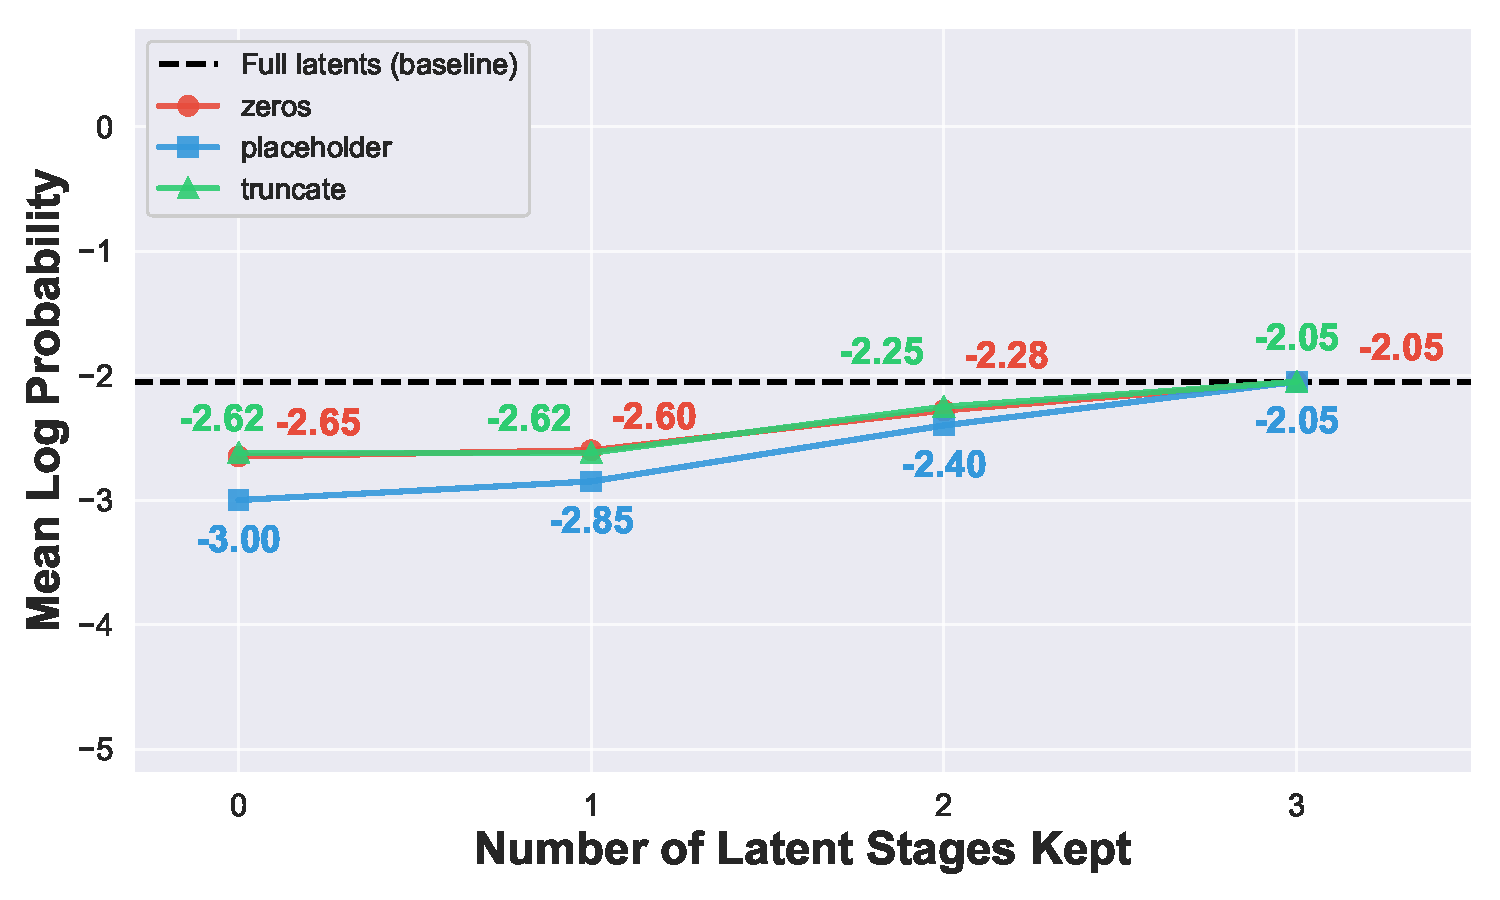
\includegraphics[width=0.49\textwidth]{imgs/ablation_log_probs_breathing_room.pdf}
    \caption{\textbf{Impact of latent stage ablation on answer confidence.} We measure the mean log-probability of ground-truth answers on GSM8k while progressively removing latent stages via zeroing, placeholder replacement, or truncation. The observed monotonic increase in probability as more stages are retained demonstrates that PaCT utilizes each computational stage to actively refine its final prediction.}
    \label{fig:latent_requirement_ablation}
    \vspace{-8mm}
\end{figure}


Efficiency gains would be unconvincing if latent stages acted as inert compute. We therefore test whether each
reasoning stage contributes to the final prediction by ablating entire stages at inference time. Concretely, we
progressively remove latent stages (each stage contains $L{=}2$ latent reasoning states on GSM8k) and measure the
resulting change in log-probability assigned to (i) the model’s generated answer token and (ii) the ground-truth
answer token.
Figure~\ref{fig:latent_requirement_ablation}
shows a clear monotonic trend: retaining more stages yields higher answer likelihood, and removing later stages causes
the largest confidence drops. This indicates that PaCT stages are actively used to refine the final prediction.

\subsection{Latent stage specialization and depth scaling}
\label{sec:latent_content}

\begin{table}[t]
\centering
\small
\caption{\textbf{Latent similarity diagnostics.} PaCT exhibits high within-stage similarity but low cross-stage similarity,
while Coconut exhibits the opposite trend.}
\label{tab:latent_similarity}
\begin{tabular}{lcc}
\toprule
Metric & PaCT & Coconut \\
\midrule
Within-stage cosine similarity & $0.99 \pm 0.01$ & $0.30 \pm 0.17$ \\
Cross-stage cosine similarity  & $0.31 \pm 0.21$ & $0.63 \pm 0.14$ \\
\bottomrule
\end{tabular}
\vspace{-6mm}
\end{table}

PaCT uses \emph{stage-wise resynthesis}: each stage constructs its latent states directly from the current textual
context and previously generated latent states, rather than recurrently transforming a single latent trajectory as in Coconut. Table~\ref{tab:latent_similarity}
offers a mechanistic view of this difference. In PaCT, latent states within the same stage are nearly identical (0.99
cosine similarity), while cross-stage similarity is much lower (0.31), suggesting that successive stages encode distinct
information. Coconut exhibits the reverse: within-stage latent states are diverse (0.30), but cross-stage similarity is
higher (0.63), consistent with recurrent unrolling that encourages information to be carried forward along a single evolving state. This structure has a direct implication: if within-stage latent states are largely redundant in PaCT, compute is better
allocated toward \emph{depth} (more stages) than toward \emph{width} (more latent states per stage), provided a
minimum of within-stage width is preserved to sustain the bidirectional refinement that makes each stage informative.
We validate this first in Figure~\ref{fig:accuracy_and_latent_stages}, which shows consistent gains from increasing
the number of stages across datasets, and then in Table~\ref{tab:width_depth_budget}, which fixes the total latent
budget and sweeps over width--depth splits.

\begin{figure}[t]
  \centering
  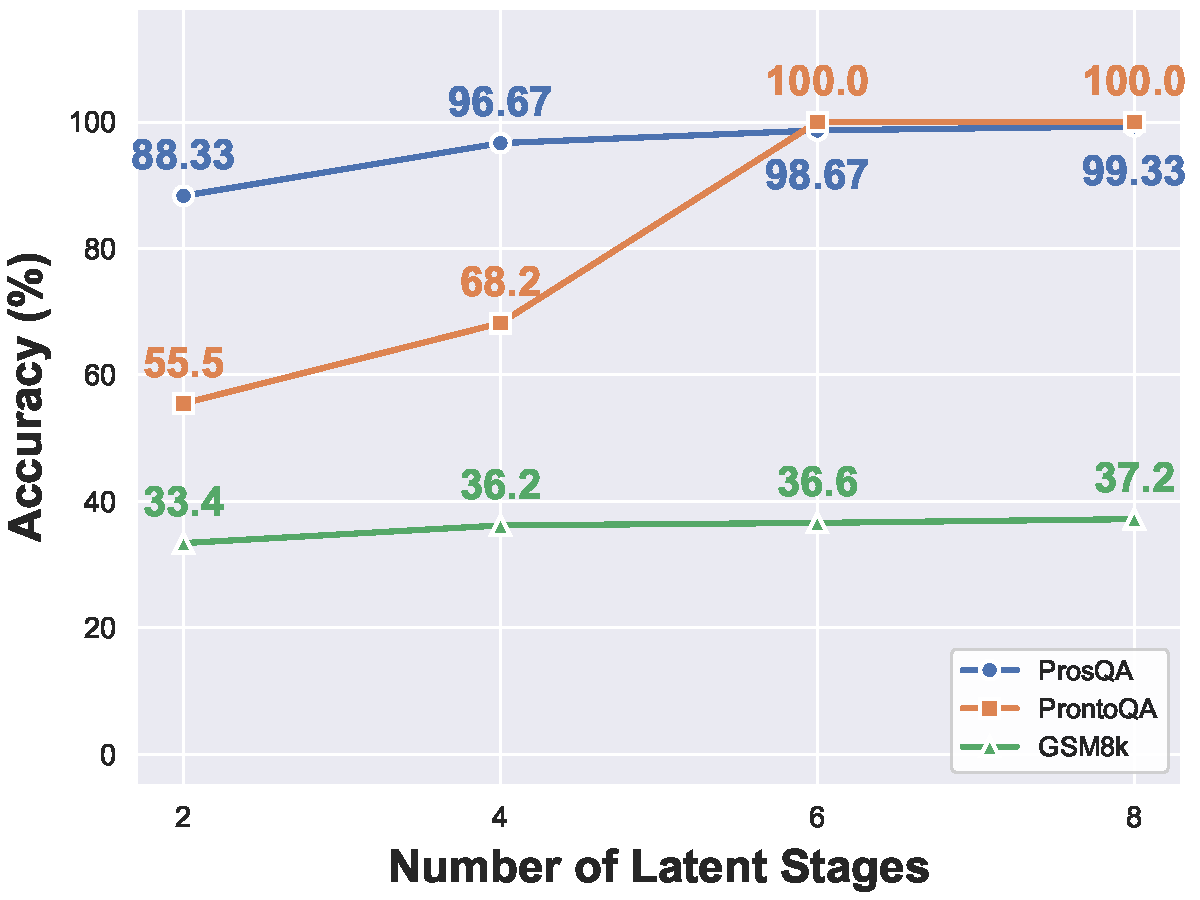
\includegraphics[width=0.8\linewidth]{imgs/table_seven_styled_values.pdf}
  \caption{\textbf{Accuracy vs.\ number of stages.} Increasing the number of latent stages improves accuracy across benchmarks.}
  \label{fig:accuracy_and_latent_stages}
\end{figure}

\paragraph{Width-depth tradeoff under a fixed latent budget.}
To disentangle the contributions of within-stage width $L$ and reasoning depth $S$, we fix the total latent budget
at $L \cdot S = 6$ on GSM8k and sweep over the four integer factorizations, keeping every other hyperparameter at
the default configuration. Table~\ref{tab:width_depth_budget} reports the resulting accuracies.

\begin{table}[t]
\centering
\small
\caption{\textbf{Width--depth allocation under a fixed latent budget.}
Holding the total number of latent reasoning states constant at $L \cdot S = 6$ on GSM8k, we vary how the budget
is split between within-stage width $L$ and reasoning depth $S$. A balanced allocation that favours depth
($L{=}2$, $S{=}3$) is best; both pure width ($S{=}1$) and pure depth ($L{=}1$) underperform.}
\label{tab:width_depth_budget}
\begin{tabular}{ccc}
\toprule
Width $L$ & Depth $S$ & Accuracy (\%) \\
\midrule
6 & 1 & 26.0 \\
3 & 2 & 30.0 \\
\textbf{2} & \textbf{3} & \textbf{34.4} \\
1 & 6 & 29.6 \\
\bottomrule
\end{tabular}
\end{table}

The sweep reveals a clearly non-monotonic pattern. Placing the entire budget in width with a single reasoning stage
($L{=}6$, $S{=}1$) performs worst ($26.0\%$), confirming that PaCT's gains are not driven by within-stage latent
quantity: beyond a small $L$, additional within-stage states are redundant. Depth therefore matters — all
multi-stage configurations outperform $S{=}1$. However, collapsing width entirely to a single latent per stage
($L{=}1$, $S{=}6$) also degrades performance ($29.6\%$), because the bidirectional refinement introduced in
Sec.~\ref{sec:latent_refinement} requires at least two within-stage latents to act on. The balanced allocation
($L{=}2$, $S{=}3$, matching our default in Table~\ref{tab:main_results}) attains the best accuracy ($34.4\%$).
The broader conclusion is that depth dominates width, but a minimal amount of within-stage width ($L \ge 2$) is
necessary to realise the benefits of stage-wise bidirectional refinement — consistent with the within-stage
similarity structure in Table~\ref{tab:latent_similarity} and with the submanifold structure documented later in
Sec.~\ref{sec:perturbation_analysis}.

\subsection{Latent token decoding analysis}
\label{sec:latent_decoding}

Although PaCT latent states are not trained to be decoded as language, we can obtain a coarse qualitative probe by
projecting each latent embedding into vocabulary space and inspecting the top predicted token at that latent position
after the Transformer pass. This probe is not meant to claim that latents are ``natural language''; rather, it helps
visualize whether the model’s internal trajectory moves from intermediate quantities toward the final answer.

\begin{table}[t]
\centering
\small
\caption{\textbf{Final-latent confidence for correct vs.\ incorrect predictions.} Top-1 probability at the final latent
position.}
\label{tab:latent_confidence}
\begin{tabular}{lcc}
\toprule
Model & Correct & Incorrect \\
\midrule
PaCT    & $0.680 \pm 0.315$ & $0.257 \pm 0.223$ \\
Coconut & $0.744 \pm 0.244$ & $0.312 \pm 0.232$ \\
\bottomrule
\end{tabular}
\vspace{-5mm}
\end{table}

Table~\ref{tab:latent_confidence} shows that the final latent’s top-1 probability separates correct from incorrect predictions, indicating that latent trajectories carry a meaningful confidence signal. Figure~\ref{fig:latent_examples} illustrates two representative cases: in correct predictions, decoded latents progress from intermediate quantities to the final answer with sharpening confidence, while in incorrect predictions the model identifies partial intermediates but fails to compose them correctly. Additional examples and related analyses comparing single-latent PaCT to double-latent Coconut are provided in \ref{subsec:latent_redundancy} and \ref{sec:single_double} respectively. An algorithm of the probing process can be found in \ref{alg:latent_probe_topk}.
\begin{figure}[t]
\centering
\fbox{%
\parbox{0.94\columnwidth}{
\textbf{Example 1} \hfill \textcolor{green!60!black}{\textbf{Correct}} \\[0.4em]
\textbf{Question:} Kenny played basketball last week. He ran for twice as long as he played basketball, and he practiced on the trumpet for twice as long as he ran. If he practiced on the trumpet for 40 hours, how many hours did Kenny play basketball? \\[0.2em]
\textbf{Ground Truth CoT:} $40 \div 2 = 20 \rightarrow 20 \div 2 = 10$ \\[0.2em]
\textbf{Predicted:} 10 \quad \textbf{GT:} 10 \\[0.4em]
\begin{tabular}{c|cccccc}
& L0 & L1 & L2 & L3 & L4 & L5 \\
\hline
Token & \textbf{20} & \textbf{20} & \textbf{10} & \textbf{10} & \textbf{10} & \textbf{10} \\
Prob  & 4.7\% & 6.8\% & 15\% & 31\% & 95\% & 94\% \\
\end{tabular} \\[-0.3em]
\textit{Interpretation:} Latents capture the intermediate (20) then converge to the final answer (10) with sharp confidence increases.
}}



\caption{\textbf{Representative decoded latent trajectories.} Within-stage latent pairs often decode to identical tokens,
consistent with high within-stage similarity in Table~\ref{tab:latent_similarity}. Additional examples are provided in
Appendix~ \ref{app:latent_decoding_examples}.}
\label{fig:latent_examples}
\end{figure}

\subsection{PaCT promotes stable latent dynamics}
\label{sec:icr_analysis}

\begin{figure}[t]
  \centering
  
\includegraphics[width=\linewidth]{imgs/icr_plot.pdf}
  \caption{\textbf{Layer-wise difference in ICR scores between PaCT and Coconut.} Negative values indicate lower ICR for PaCT.}
  \label{fig:icr}
  \vspace{-6mm}
\end{figure}

Beyond accuracy and efficiency, we examine how PaCT alters internal reasoning dynamics. We analyze hidden representations using the Information Contribution to the Residual Stream (ICR) score~\cite{zhang2025icr}, which measures deviation of residual updates from attention-based explanations. Figure~\ref{fig:icr} shows consistently lower ICR for PaCT in the middle layers, indicating earlier stabilization relative to Coconut. This aligns with PaCT’s stage-wise latent resynthesis, where each stage is grounded in the current context rather than accumulating latent history through recurrent unrolling.


\subsection{Effect of context length for latent synthesis}
\label{subsec:context_length}

\begin{table}[t]
    \centering
    \small
    \caption{Effect of number of context tokens on PaCT (GPT-2) performance on GSM8k.}
    \label{tab:gpt2_gsm8k_context}
    \begin{tabular}{cc}
        \toprule
        {Number of context tokens} & Accuracy \\
        \midrule
         2   & 34.4 \\
         4   & 33.0 \\
         8   & 32.3 \\
         All & 30.6 \\
        \bottomrule
    \end{tabular}
\end{table}

\begin{figure}[t]
    \centering
    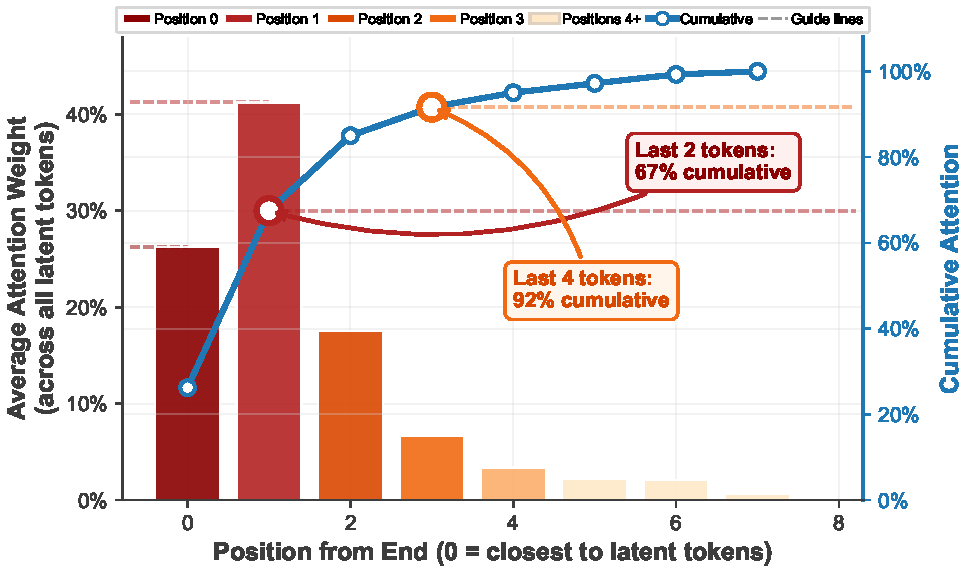
\includegraphics[width=\linewidth]{imgs/cross_attention_bias.pdf}
    \caption{\textbf{Cross-attention weight distribution across different number of context tokens.}
    Position 0 denotes the \textbf{last} token before latent synthesis, position 1 the \textbf{second-to-last}, and so on.
    The model concentrates attention on the most recent 1--2 positions regardless of available context.}
    \label{fig:attention_heatmap}
    \vspace{-5mm}
\end{figure}


A key design choice in PaCT is the number of context tokens used as keys and values for cross-attention
during latent synthesis. Table~\ref{tab:gpt2_gsm8k_context} shows that expanding this context beyond a
small window does not improve performance and can even degrade it. Figure~\ref{fig:attention_heatmap}
explains this behavior: regardless of available context length, cross-attention concentrates on the most
recent hidden states.

This aligns with prior observations that Transformer attention exhibits a strong inductive bias toward
recency~\citep{press2021train}. In PaCT, this bias is amplified because latent synthesis attends not only
to text tokens but also to latent states from previous stages, which already summarize the cumulative
context. As a result, attending to recent latents provides access to relevant historical information
without requiring long text-level context.

Together, these results justify a restricted context window for latent synthesis, which aligns with the
model’s learned attention bias while improving computational efficiency.


\subsection{Perturbing PaCT's latent states}
\label{sec:perturbation_analysis}

Having established that each reasoning stage contributes to PaCT's final prediction
(Sec.~\ref{sec:stage_ablation}) and that latent trajectories carry a meaningful confidence signal
(Sec.~\ref{sec:latent_decoding}), we now probe what the latent reasoning states actually encode by
intervening on them directly at inference time. The guiding hypothesis is simple: if the latents
carry task-relevant reasoning information, destructive perturbations that erase or replace them
should reduce accuracy substantially, whereas structure-preserving noise should be largely absorbed.

\paragraph{Probes.}
We apply five inference-time interventions to a trained PaCT model on GSM8k, without any additional
training: (i) \emph{zeroing}, where every latent state is replaced with the zero vector;
(ii) \emph{random-norm replacement}, where each latent is replaced with a Gaussian random vector
rescaled to match the empirical latent norm; (iii) \emph{cross-example swap}, where latents
synthesized for a randomly paired, unrelated example are substituted for the current ones;
(iv) \emph{no-prompt decode}, where answer tokens are prevented from attending back to the question
prefix during decoding so that the answer must be reconstructed from the latent states alone; and
(v) \emph{additive Gaussian noise} $\varepsilon \sim \mathcal{N}(0, \sigma^2 I)$ added to every
latent, swept over $\sigma \in \{0.01, 0.05, 0.1, 1.0\}$.

\begin{table}[t]
\centering
\small
\caption{\textbf{Perturbing PaCT's latent reasoning states on GSM8k.}
Destructive interventions (zeroing, random-norm replacement, cross-example swap) collapse accuracy,
while structure-preserving Gaussian noise is largely absorbed. Restricting answer decoding to attend
only to latent states (no-prompt decode) also collapses accuracy, indicating that the latents encode
information not redundantly present in the prompt.}
\label{tab:latent_perturbation}
\begin{tabular}{@{}lc@{}}
\toprule
Condition & Accuracy (\%) \\
\midrule
PaCT (clean)                                        & 34.40 \\
\midrule
Zero all latents                                    & 7.80  \\
Random vectors, matched norm                        & 8.77  \\
Swap latents across examples                        & 4.27  \\
No-prompt decode (answer attends only to latents)   & 7.40  \\
\midrule
Gaussian noise, $\sigma{=}0.01$                     & 33.62 \\
Gaussian noise, $\sigma{=}0.05$                     & 33.62 \\
Gaussian noise, $\sigma{=}0.10$                     & 33.78 \\
Gaussian noise, $\sigma{=}1.00$                     & 31.77 \\
\bottomrule
\end{tabular}
\end{table}

Table~\ref{tab:latent_perturbation} summarizes the results. Three observations follow.
\emph{First, destructive perturbations collapse performance.} Zeroing ($7.80\%$), random-norm
replacement ($8.77\%$), and cross-example swap ($4.27\%$) each reduce accuracy by more than $25$
absolute points from the $34.40\%$ clean baseline, so the latent states are load-bearing for PaCT's
predictions rather than acting as passive padding.
\emph{Second, the latent pathway carries non-redundant information.} When answer decoding is
restricted to attend only to the latent states, accuracy falls to $7.40\%$, showing that the latents
encode signal that the prompt path alone cannot reconstruct.
\emph{Third, latents occupy a structured submanifold.} Gaussian perturbations stay close to the
clean baseline across the entire sweep ($33.62\%$ at $\sigma{=}0.01$, $33.62\%$ at $\sigma{=}0.05$,
$33.78\%$ at $\sigma{=}0.1$, and $31.77\%$ even at $\sigma{=}1.0$), whereas random unit-norm
replacements — which share the noise's isotropy but destroy the learned directions — collapse it
($8.77\%$). The latents therefore live on a learned submanifold along which small,
structure-preserving perturbations are absorbed, while arbitrary high-magnitude directions are not.
These probes are run at the GPT-2 scale on GSM8k.

\subsection{Out-of-distribution generalization}
\label{sec:ood_transfer}

To assess whether PaCT's improvements on GSM8k reflect genuine arithmetic reasoning rather than
GSM8k-specific regularities, we evaluate GSM8k-trained checkpoints zero-shot on three held-out math
benchmarks: GSM-HARD, MultiArith, and SVAMP. Coconut results are obtained by rerunning the released
Coconut~\cite{hao2024training} implementation under its best reported configuration for this
setting, and for MultiArith we use the same evaluation subset adopted in prior continuous latent
reasoning work, ensuring an apples-to-apples comparison.

\begin{table}[t]
\centering
\small
\caption{\textbf{Out-of-distribution generalization.}
All models are trained on GSM8k and evaluated zero-shot on three held-out math benchmarks. PaCT
matches or exceeds Coconut on every split.}
\label{tab:ood_transfer}
\begin{tabular}{lcc}
\toprule
Dataset & PaCT (\%) & Coconut (\%) \\
\midrule
GSM-HARD                  & \textbf{7.88}  & 7.90  \\
MultiArith                & \textbf{82.34} & 82.00 \\
SVAMP                     & \textbf{37.67} & 36.40 \\
\bottomrule
\end{tabular}
\end{table}

As shown in Table~\ref{tab:ood_transfer}, PaCT matches or exceeds Coconut across all three OOD
benchmarks. This suggests that the improvements observed on GSM8k translate to related but held-out
distributions rather than being tied to GSM8k-specific artifacts.


% ###################################################################
% ###################################################################
% ###################################################################


